\chapter{Substrate-Independency}

\label{chap:woodensimulation}
\index{Wooden Turing Machine}

The brain of a computer---its central processing unit (CPU)---consists of a set of electronic switches called transistors.
However, a CPU does not need to be an electronic device. One could just as easily implement the required logic using a set of wooden gates, for example.

In theory, one could implement a DNA simulation on a mechanically operated computer composed of wooden components.
Instead of using transistors on a silicon chip to control electrons, one could use wooden gates on a plywood platform to control wooden balls.
As such a machine stepped through its logic, a virtual human would take its first steps in its virtual universe.

What is this strange phenomenon that creates consciousness and pain from a clacking pile of wooden pieces?

If a vast number of moving wooden components can create pain, what does a single moving piece of wood create? 

If huge number of flipping bits generate conscious and pain, what does one bit flip describe?

If Turing Machine with astronomically many symbols create consciousness and pain, then what does one symbol create?

Can contemporary physics even describe this process?

It can't. Such an real-virtual action would require metaphysics to be explained, which would be a contradiction 
with the initial axioms.

The only logical conclusion is that the relation is not causal, but representational. A flipping bits (simulator) and the corresponding simulation
(consciousness and pain) are two sides of the same coin - they are two arrangements  of the same information.




No man-made device is perfect, and a wooden Turing machine is no exception. Friction, mechanical tolerances, and similar physical factors introduce resonances and unintentional vibrations into its operation. If the intended logic inside the wooden Turing machine creates a virtual universe filled with pain and consciousness, what do these unintentional side effects create? Do they manifest in some form within the virtual world as well?

Would a virtual inhabitant in that universe discover them as a form of quantum foam? Might they observe them as cosmic microwave background radiation at a temperature of 2.725\,K?

Perhaps so. At the very least, it would be difficult to argue why the macro-movements of wooden components should count toward the simulation while their microscopic resonances do not.

How would the clock speed of the machine running the simulation appear to the simulated entity? Would they observe that particles in their universe seem to follow a strange, abstract square wave function---one whose origin they cannot explain, but which they might end up calling the Wintel\texttrademark\ abstract square wave function?

Beyond Turing machines, it is easy to imagine other physical systems generating virtual universes. One potential medium for consciousness could be the surface of the sea. In theory, ocean waves and ripples could execute a DNA simulation in which conscious observers marvel at the wonderful properties of their universe (such as those brought on by heavy rainfall during the annual monsoon season).

One could also use a thermostat to represent any procedure by controlling temperature over time. As the temperature varies, the thermostat could step through the binary code of the DNA simulation. Of course, the simulated entity would be entirely unaware that a trivial thermostat was responsible for the illusion of its existence. Naturally, the thermostat itself cannot be considered conscious by any stretch of the imagination.

Correspondingly, running such DNA simulations on any type of computer does not make the physical computer itself conscious or sensitive to pain. It remains a simple Turing machine stepping through its tape of symbols, lacking any capacity to do otherwise. However, the executing Turing machine creates a parallel virtual universe in which a conscious human contemplates questions of free will.

The entire universe, with all its planets and stars, could itself be the substrate of a consciousness.

What do five billion human beings create as they walk along streets and pass through doorways on their way to work? For instance, a person walking through two consecutive doors implements a logical \texttt{AND} operation. If a person can pass through using either a left or a right door, they implement an \texttt{OR} operation.

Could a simple pencil and piece of paper be the substrate of consciousness? Start writing down the algorithmic evolution of DNA with a pencil, and before long, virtual people will suffer toothaches in their virtual universe. Both a graphite pencil and a ballpoint pen should work equally well---though due to higher friction, the temperature of the cosmic background radiation in a universe created by pencil might end up slightly higher!

Thus, whether we manipulate electrons or wooden components, we can construct virtual universes that mirror the structural complexity of our own. Because a simulated entity would be a virtual duplicate of its real-world counterpart, it too will eventually begin exploring its universe (just as we did). It will discover that it can build mechanisms like Turing machines, construct one, and simulate its own existence. The procedure the virtual entity uses to simulate its existence is identical to the procedure we used to create the first level of simulation. In other words:
\begin{equation*}
  \text{virtual}_1 = \text{DNA}(\text{virtual}_0)
\end{equation*}

This stack of nested simulations could theoretically continue indefinitely, or at least until a sub-simulation lacks sufficient information density to host yet another simulation layer. We know that both the virtual entity we created in our simulation and the secondary entity created by our simulation are inherently virtual. We know this because we generated them within a deterministic Turing machine whose operations are fully understood. Therefore, these recursive stages can be unified into a single expression:
\begin{equation*}
  r_{n+1} = \text{DNA}(r_n)
\end{equation*}

The axiomatic $\text{DNA}()$ procedure that maps our reality $r_n$ to a virtual world $r_{n+1}$ is identical to the procedure that maps $r_{n+1}$ to $r_{n+2}$. There is no unique parameter in this equation that distinguishes us as "real" compared to simulated entities. The only logical conclusion is that our universe is just as virtual in nature as the universes we synthesize inside our computers. In recursive procedures, it is remarkably difficult to argue that one specific level of recursion is inherently more "real" than any other. Just like the simulated entities we create, we simply do not directly perceive the virtual nature of our own reality.

\begin{figure}[htbp]
  \centering
  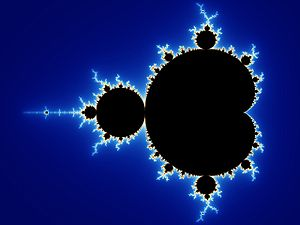
\includegraphics[width=0.8\textwidth]{figures/fractals.jpg}
  \caption{Recursion}
  \label{fig:recursion}
\end{figure}

There is, however, one glaring challenge facing the simulation hypothesis: information capacity and entropy. Simulating even a single strand of human DNA is a daunting computational task, let alone an entire human being. There are over eight billion of us, not to mention countless animals, plants, and microorganisms. Our Milky Way galaxy alone contains hundreds of billions of stars, and astronomers have observed hundreds of billions of galaxies.

Sub-simulations would rapidly run out of memory!

Despite their purely virtual nature, these abstract structures possess fascinating properties.
Subjective pain and joy are profoundly real experiences for conscious beings.
Could there be fundamental modes of feeling that biological evolution has simply not implemented in us yet?
Might we experience them if we ultimately end up in a realm like heaven?

(According to my wife, such undiscovered human experiences could certainly explain my typical behavior--I'm obviously running all of
those procedures simultaneously)

In Arnold Schwarzenegger's film \textit{Last Action Hero}, characters cross back and forth between the real world and a fictional film universe.
I never liked the movie because the premise felt far too absurd to me. Silly me.


